\chapter{Traçados sob interferência de rede elétrica}
\label{ap:figurasRuido}

Este apêndice reúne os traçados das seis classes de estímulo sob a interferência de rede de 60~Hz na amplitude de 30\,\% da excursão --- a única condição, entre as 54 avaliadas na décima quarta bateria, em que o sistema falha (Seção~\ref{sec:resBateria14}). As figuras são apresentadas em duas versões complementares.

A primeira versão (Figuras~\ref{fig:ruidoSimplesNormal} a~\ref{fig:ruidoSimplesParada}) confronta o estímulo limpo com o mesmo estímulo perturbado, na mesma escala vertical, e destina-se a documentar o material efetivamente reproduzido pelo gerador. A amplitude da perturbação é de 0,18~V, contra um pico R de 0,97~V. Nas classes que contêm pausa, a janela de oito segundos é centrada nela.

A segunda versão (Figuras~\ref{fig:ruidoCompletoNormal} a~\ref{fig:ruidoCompletoParada}) acrescenta dois painéis analíticos: um detalhe de 1,5~s sobre um complexo QRS, que permite avaliar a relação entre a amplitude da interferência e a da onda R, e a série de intervalos R-R produzida pelo algoritmo de detecção. Este último painel foi obtido alimentando-se o algoritmo com o sinal já submetido à cascata de filtros do \textit{firmware}, de modo a reproduzir a condição de operação do dispositivo.

Cabe registrar uma observação metodológica sobre essa segunda versão. Ao contrário do que se poderia supor, a soma digital da interferência ao estímulo não reproduz, para a maioria das classes, a falha observada na bancada: apenas na taquicardia o ruído sintético basta para provocar a perda de picos R e o consequente falso bloqueio (Figura~\ref{fig:ruidoCompletoTaqui}). Nas demais, o passa-baixas de 40~Hz do \textit{firmware} rejeita a perturbação assim somada e a classificação permanece correta. A discrepância entre a simulação e a bancada motivou a investigação relatada na seção seguinte.

Todas as figuras foram produzidas pelo autor a partir dos arquivos de estímulo efetivamente reproduzidos nas décima terceira e décima quarta baterias, por meio de rotinas de geração automatizada, o que assegura sua reprodutibilidade.

\section{Estímulo limpo e perturbado}

\begin{figure}[htbp]
\centering
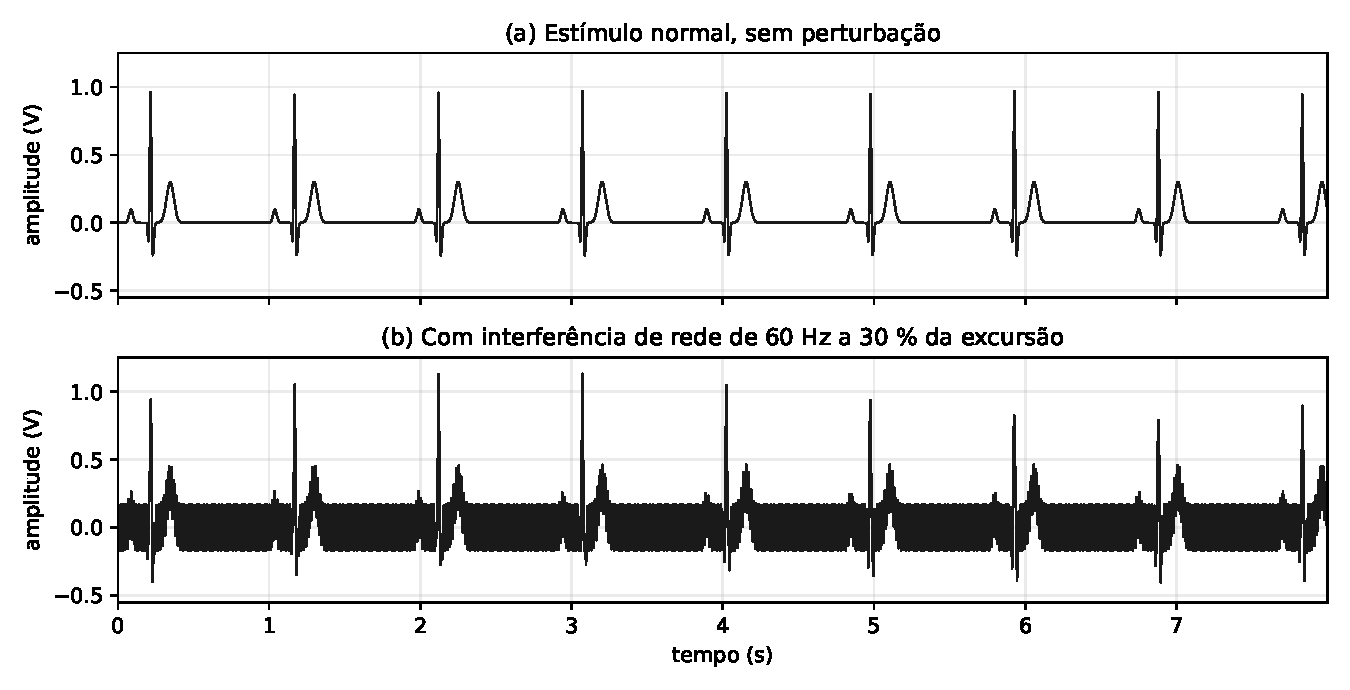
\includegraphics[width=\linewidth]{assets/figura_rede30_simples_normal.pdf}
\caption{Estímulo normal, sem e com interferência de rede de 60~Hz a 30\,\%.}
\label{fig:ruidoSimplesNormal}
\end{figure}

\begin{figure}[htbp]
\centering
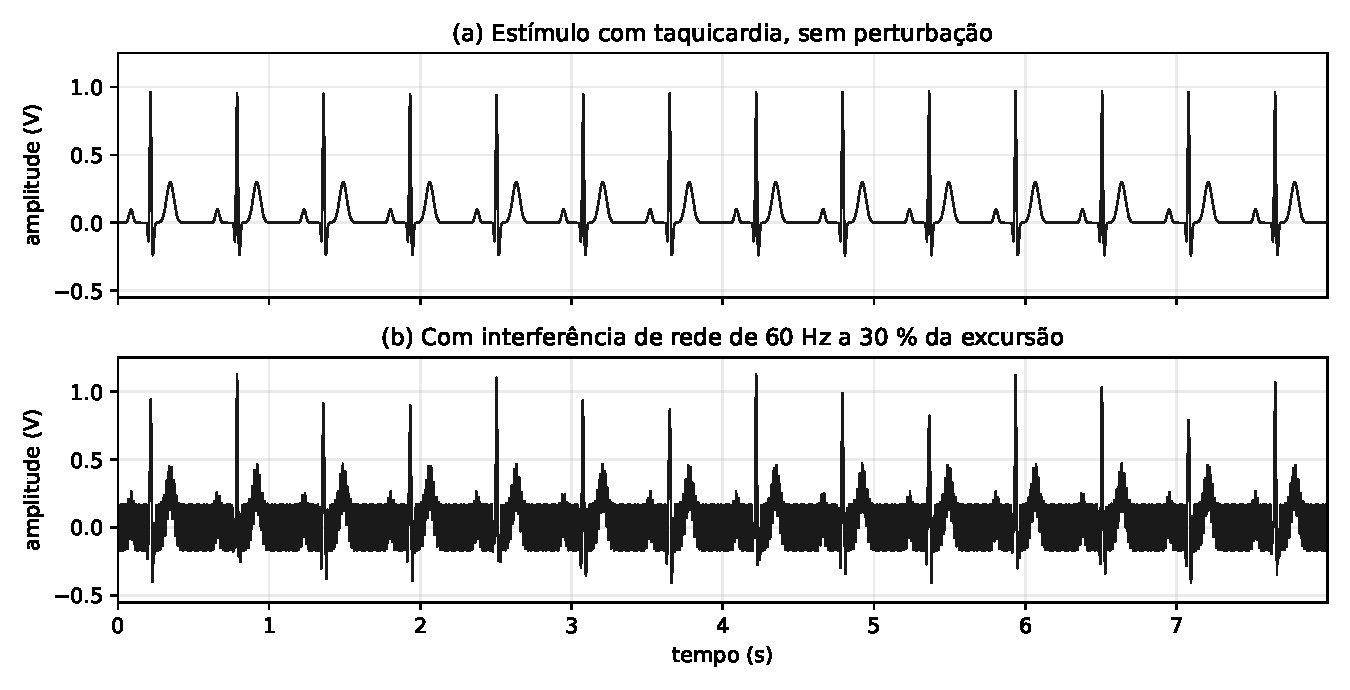
\includegraphics[width=\linewidth]{assets/figura_rede30_simples_taqui.pdf}
\caption{Estímulo com taquicardia, sem e com interferência de rede de 60~Hz a 30\,\%.}
\label{fig:ruidoSimplesTaqui}
\end{figure}

\begin{figure}[htbp]
\centering
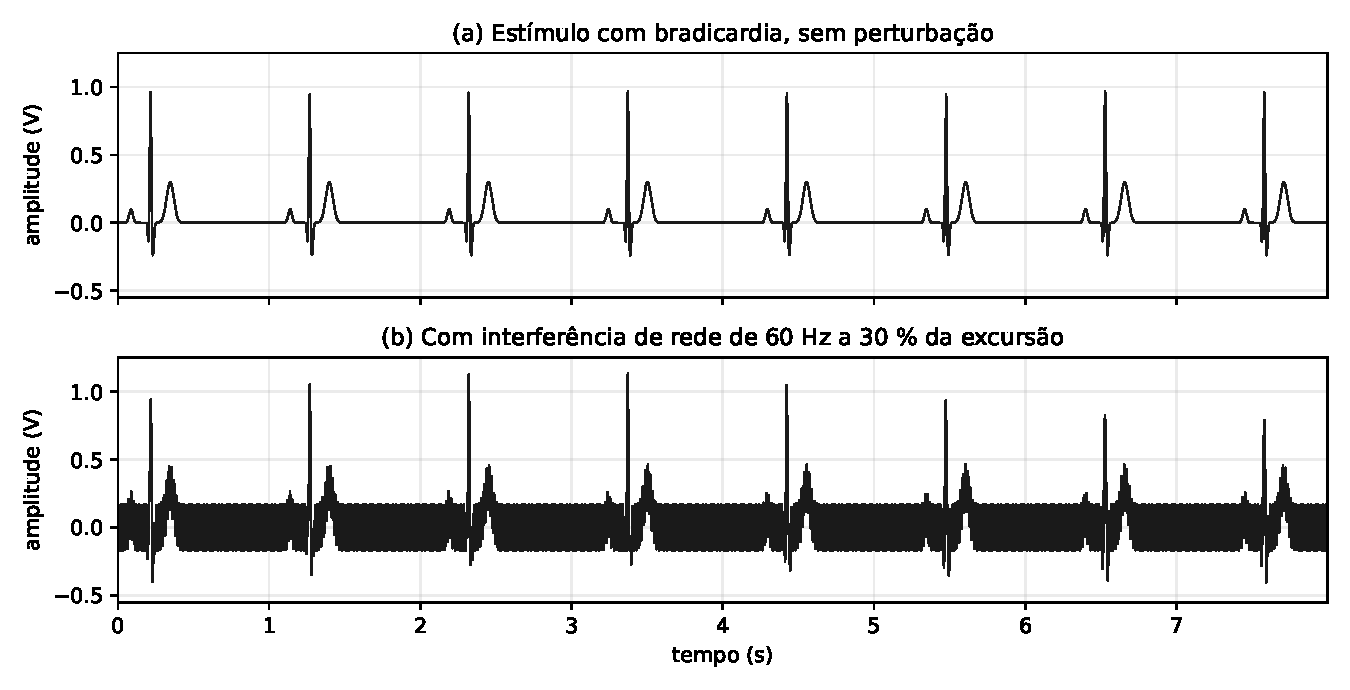
\includegraphics[width=\linewidth]{assets/figura_rede30_simples_bradi.pdf}
\caption{Estímulo com bradicardia, sem e com interferência de rede de 60~Hz a 30\,\%.}
\label{fig:ruidoSimplesBradi}
\end{figure}

\begin{figure}[htbp]
\centering
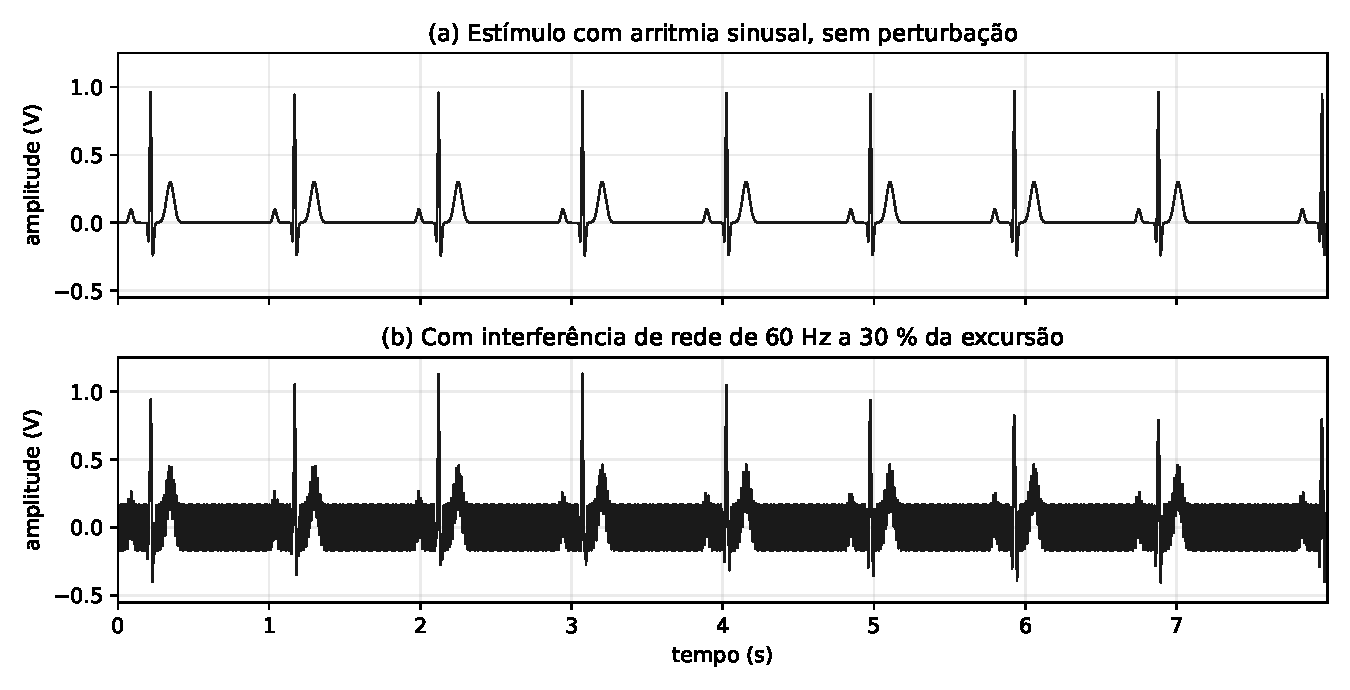
\includegraphics[width=\linewidth]{assets/figura_rede30_simples_arritmia.pdf}
\caption{Estímulo com arritmia sinusal, sem e com interferência de rede de 60~Hz a 30\,\%.}
\label{fig:ruidoSimplesArritmia}
\end{figure}

\begin{figure}[htbp]
\centering
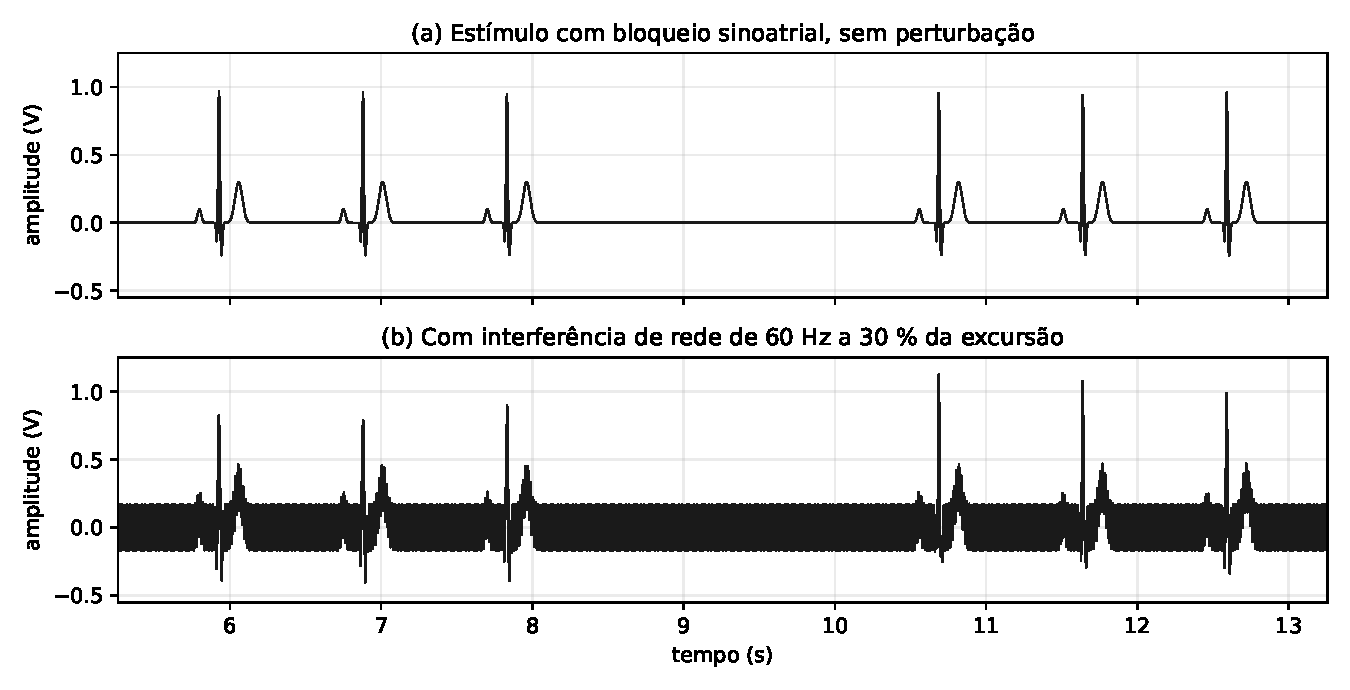
\includegraphics[width=\linewidth]{assets/figura_rede30_simples_bloqueio.pdf}
\caption{Estímulo com bloqueio sinoatrial, sem e com interferência de rede de 60~Hz a 30\,\%. A janela é centrada na pausa característica.}
\label{fig:ruidoSimplesBloqueio}
\end{figure}

\begin{figure}[htbp]
\centering
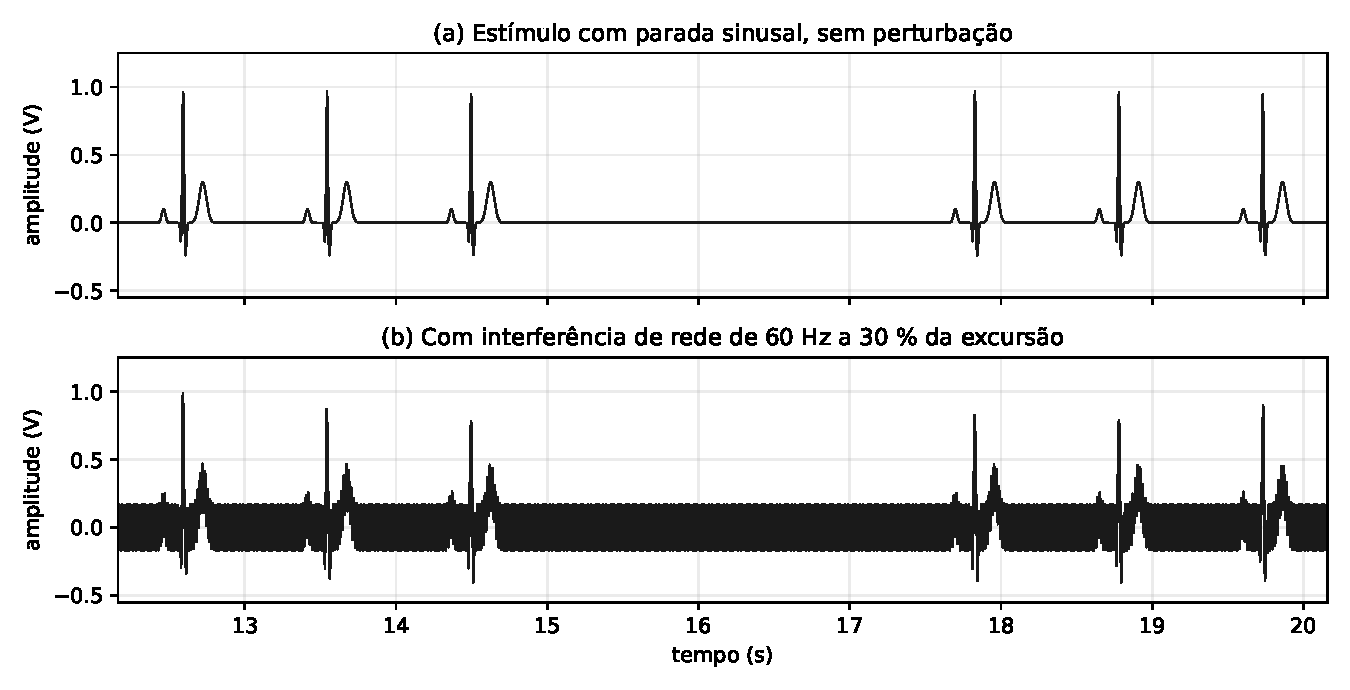
\includegraphics[width=\linewidth]{assets/figura_rede30_simples_parada.pdf}
\caption{Estímulo com parada sinusal, sem e com interferência de rede de 60~Hz a 30\,\%. A janela é centrada na pausa característica.}
\label{fig:ruidoSimplesParada}
\end{figure}

\clearpage
\section{Detalhe do complexo QRS e série de intervalos R-R}

\begin{figure}[htbp]
\centering
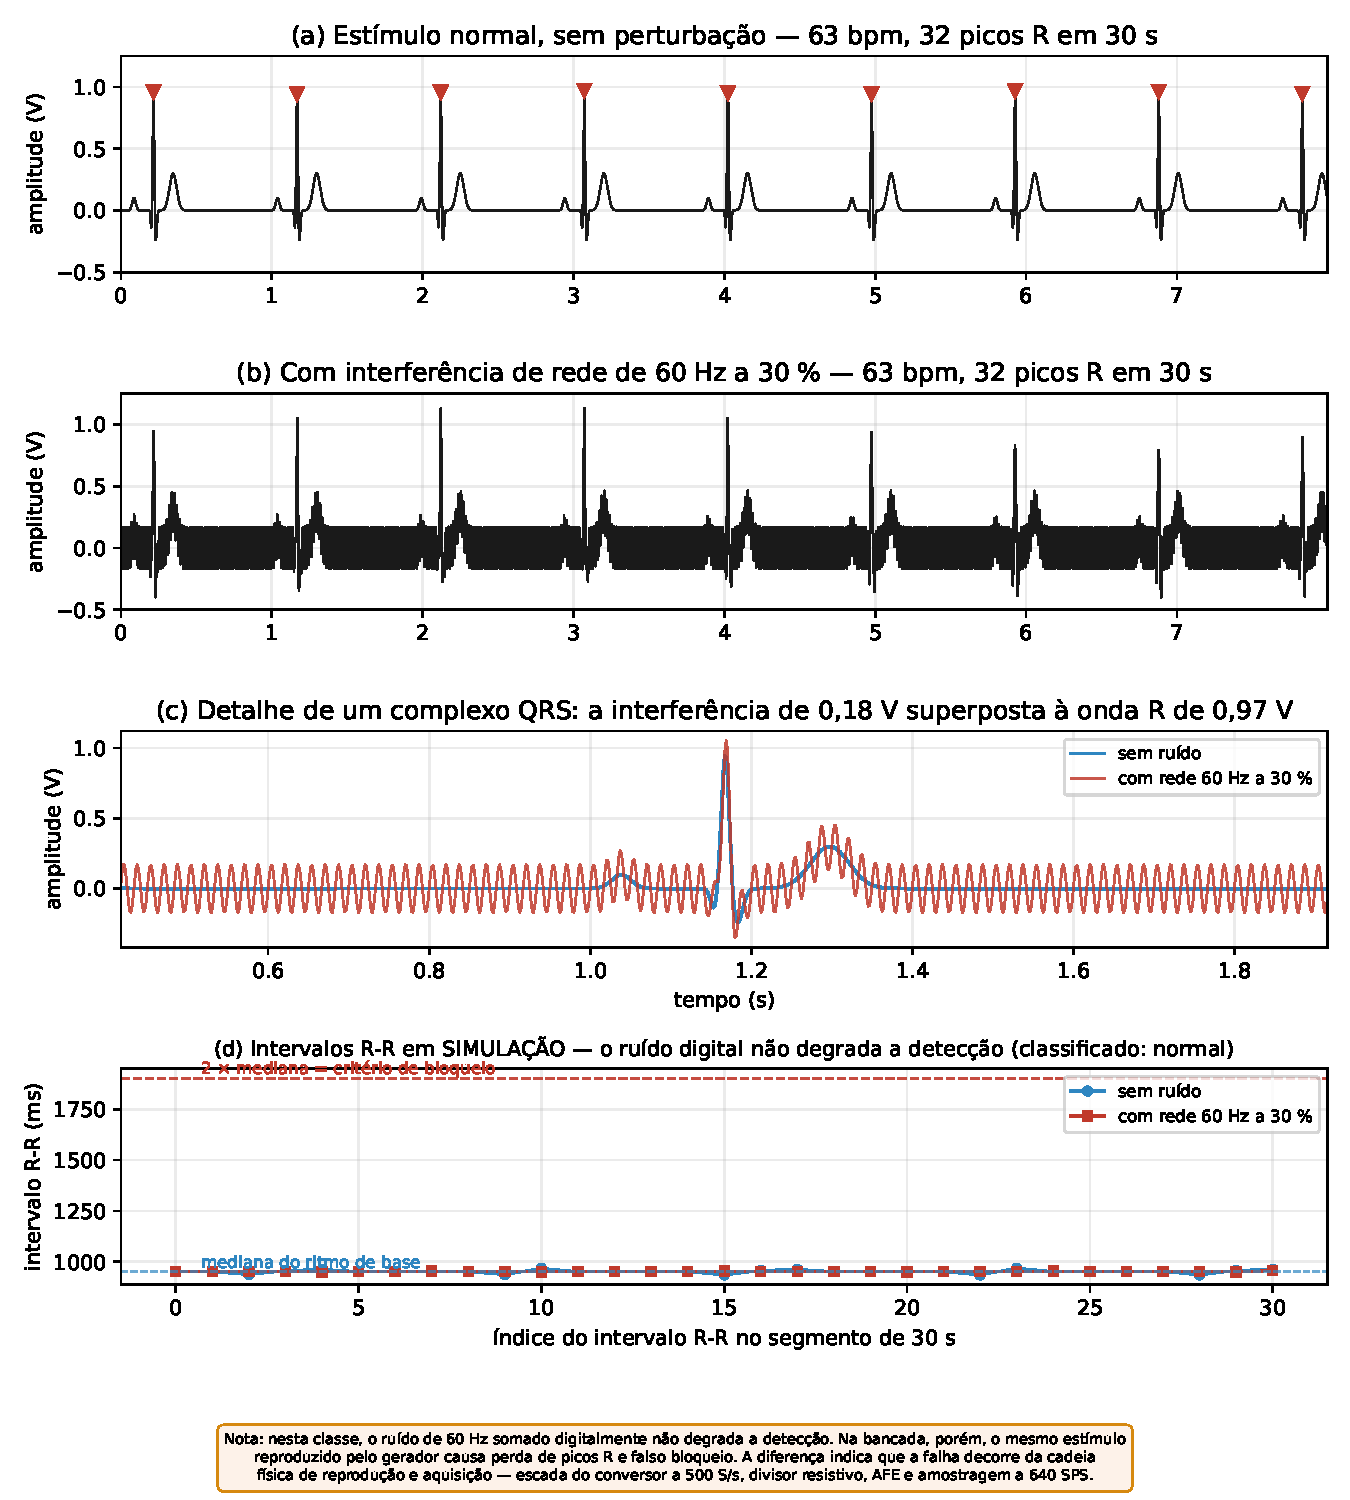
\includegraphics[width=0.92\linewidth]{assets/figura_rede30_normal.pdf}
\caption{Estímulo normal sob interferência de rede a 30\,\%: traçados, detalhe do complexo QRS e intervalos R-R.}
\label{fig:ruidoCompletoNormal}
\end{figure}

\begin{figure}[htbp]
\centering
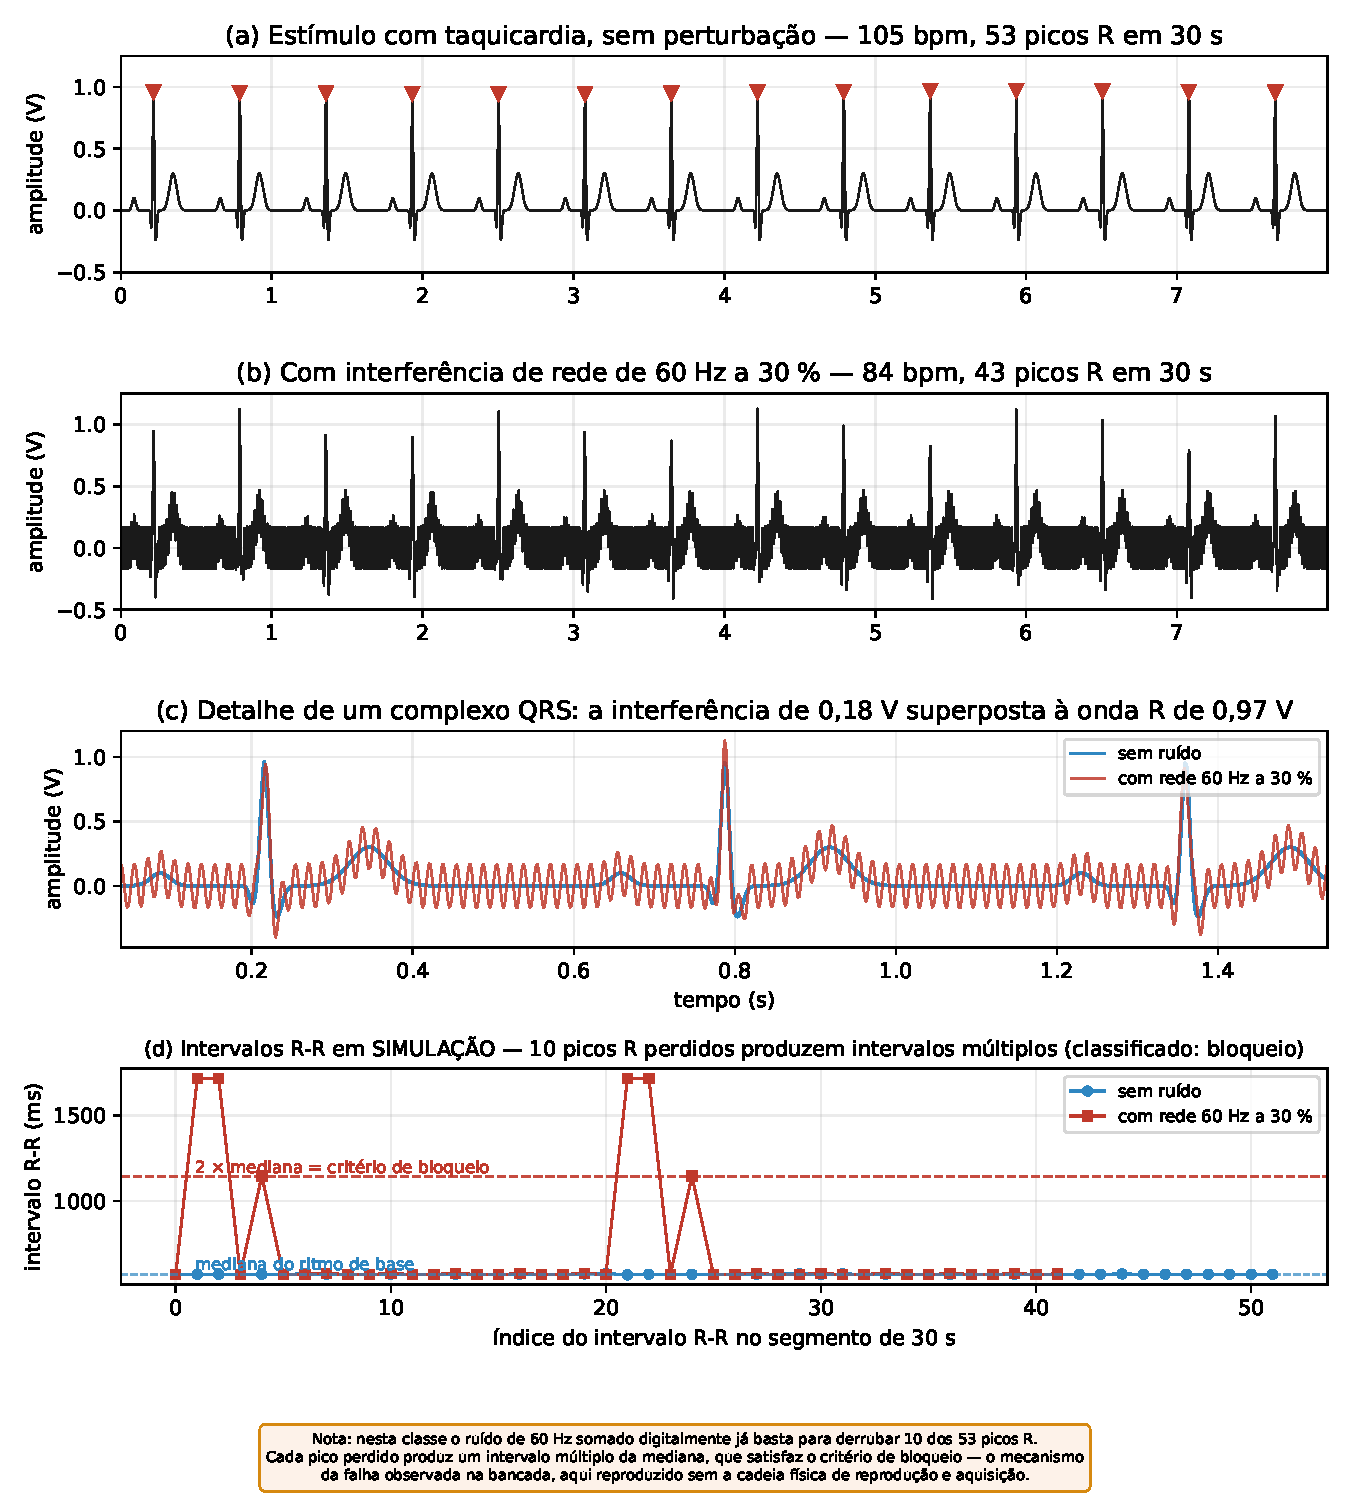
\includegraphics[width=0.92\linewidth]{assets/figura_rede30_taqui.pdf}
\caption{Estímulo com taquicardia sob interferência de rede a 30\,\%. Única classe em que a soma digital da interferência reproduz a falha observada na bancada: dez dos 53 picos R são perdidos, e cada perda produz um intervalo múltiplo do R-R de base, que satisfaz o critério de bloqueio.}
\label{fig:ruidoCompletoTaqui}
\end{figure}

\begin{figure}[htbp]
\centering
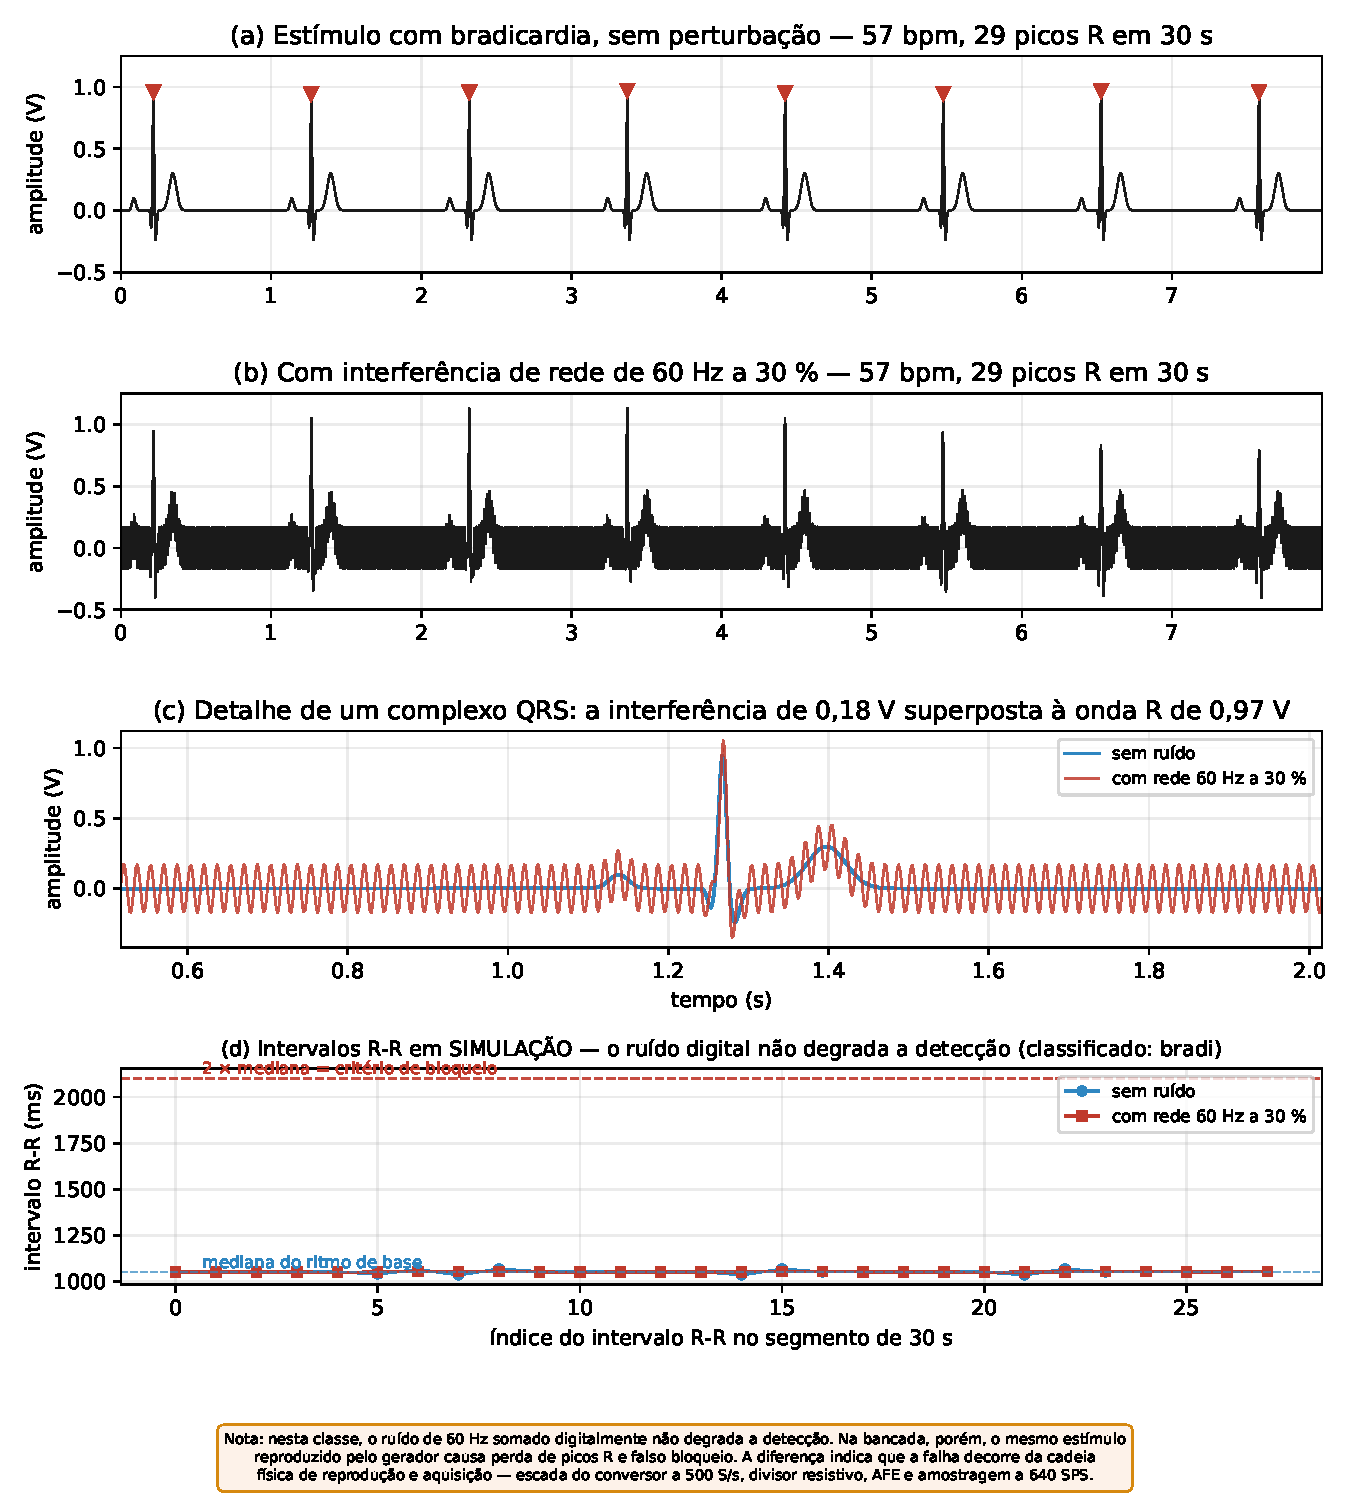
\includegraphics[width=0.92\linewidth]{assets/figura_rede30_bradi.pdf}
\caption{Estímulo com bradicardia sob interferência de rede a 30\,\%: traçados, detalhe do complexo QRS e intervalos R-R.}
\label{fig:ruidoCompletoBradi}
\end{figure}

\begin{figure}[htbp]
\centering
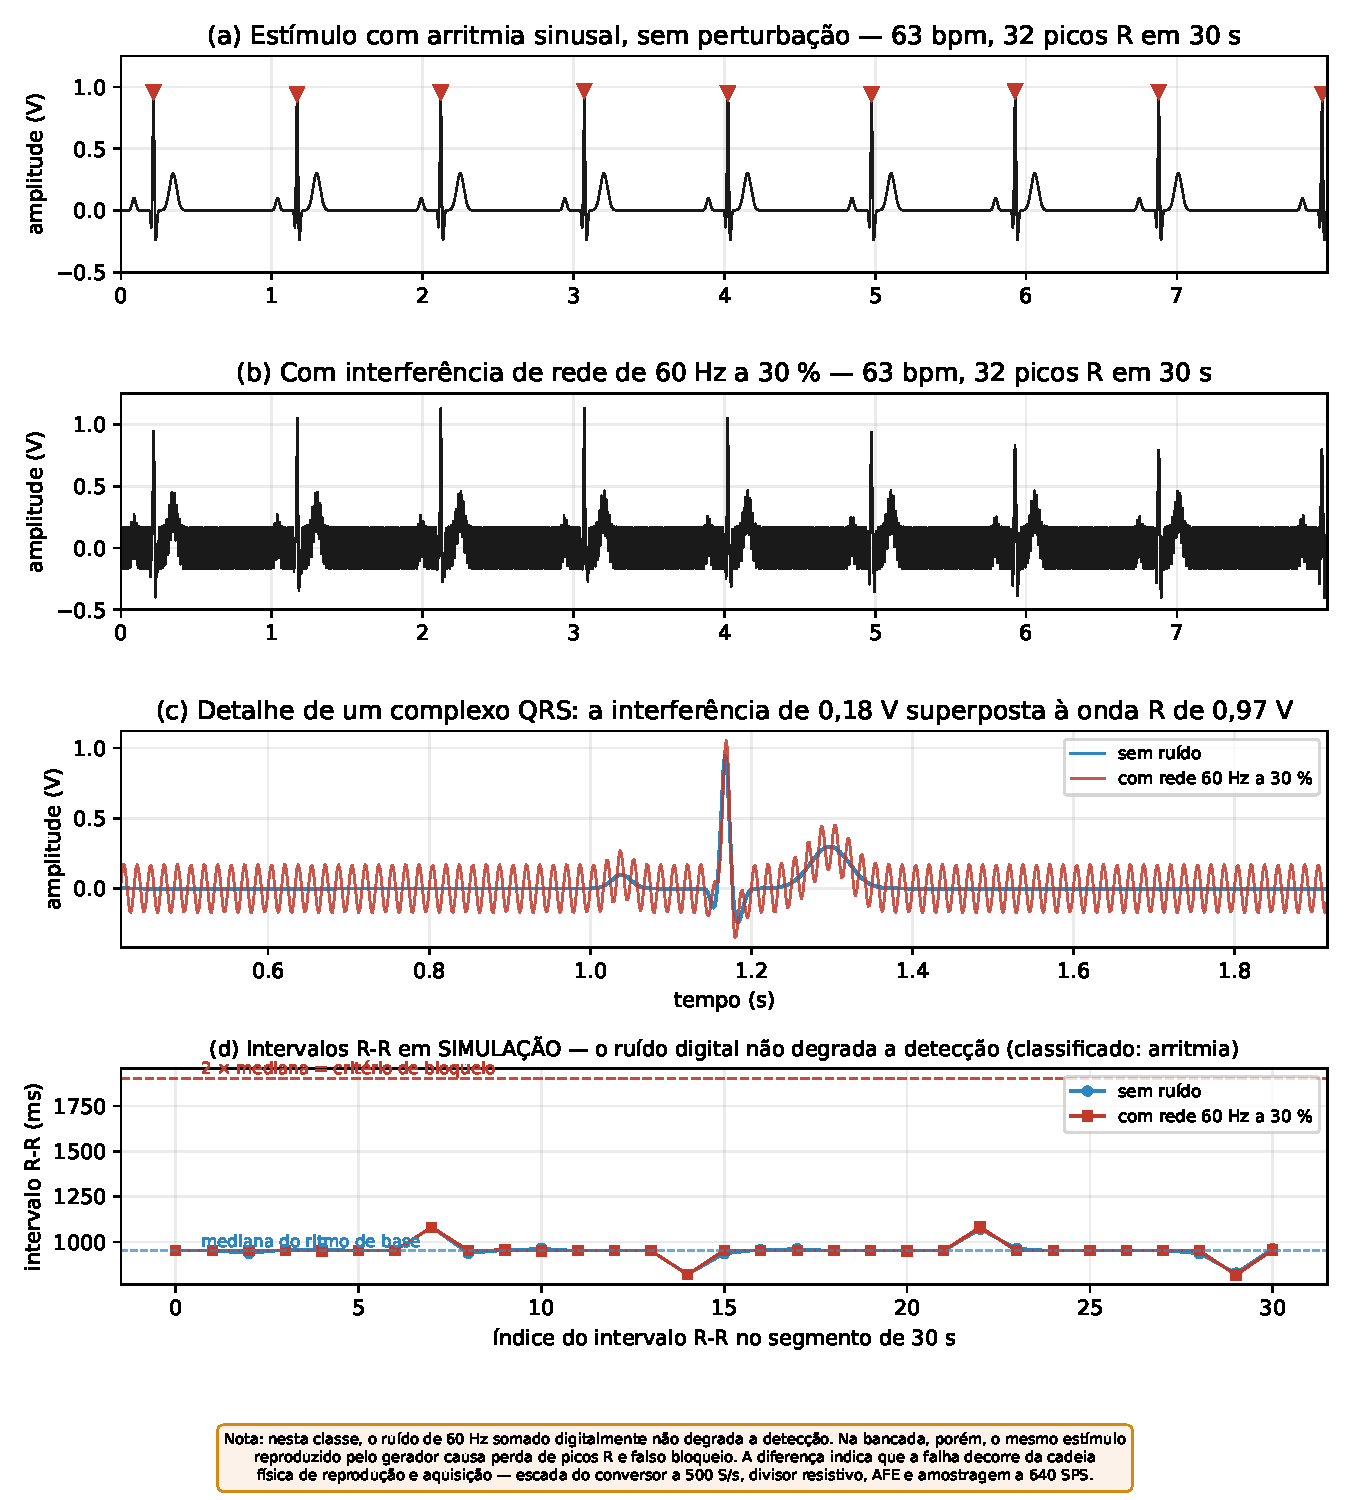
\includegraphics[width=0.92\linewidth]{assets/figura_rede30_arritmia.pdf}
\caption{Estímulo com arritmia sinusal sob interferência de rede a 30\,\%: traçados, detalhe do complexo QRS e intervalos R-R.}
\label{fig:ruidoCompletoArritmia}
\end{figure}

\begin{figure}[htbp]
\centering
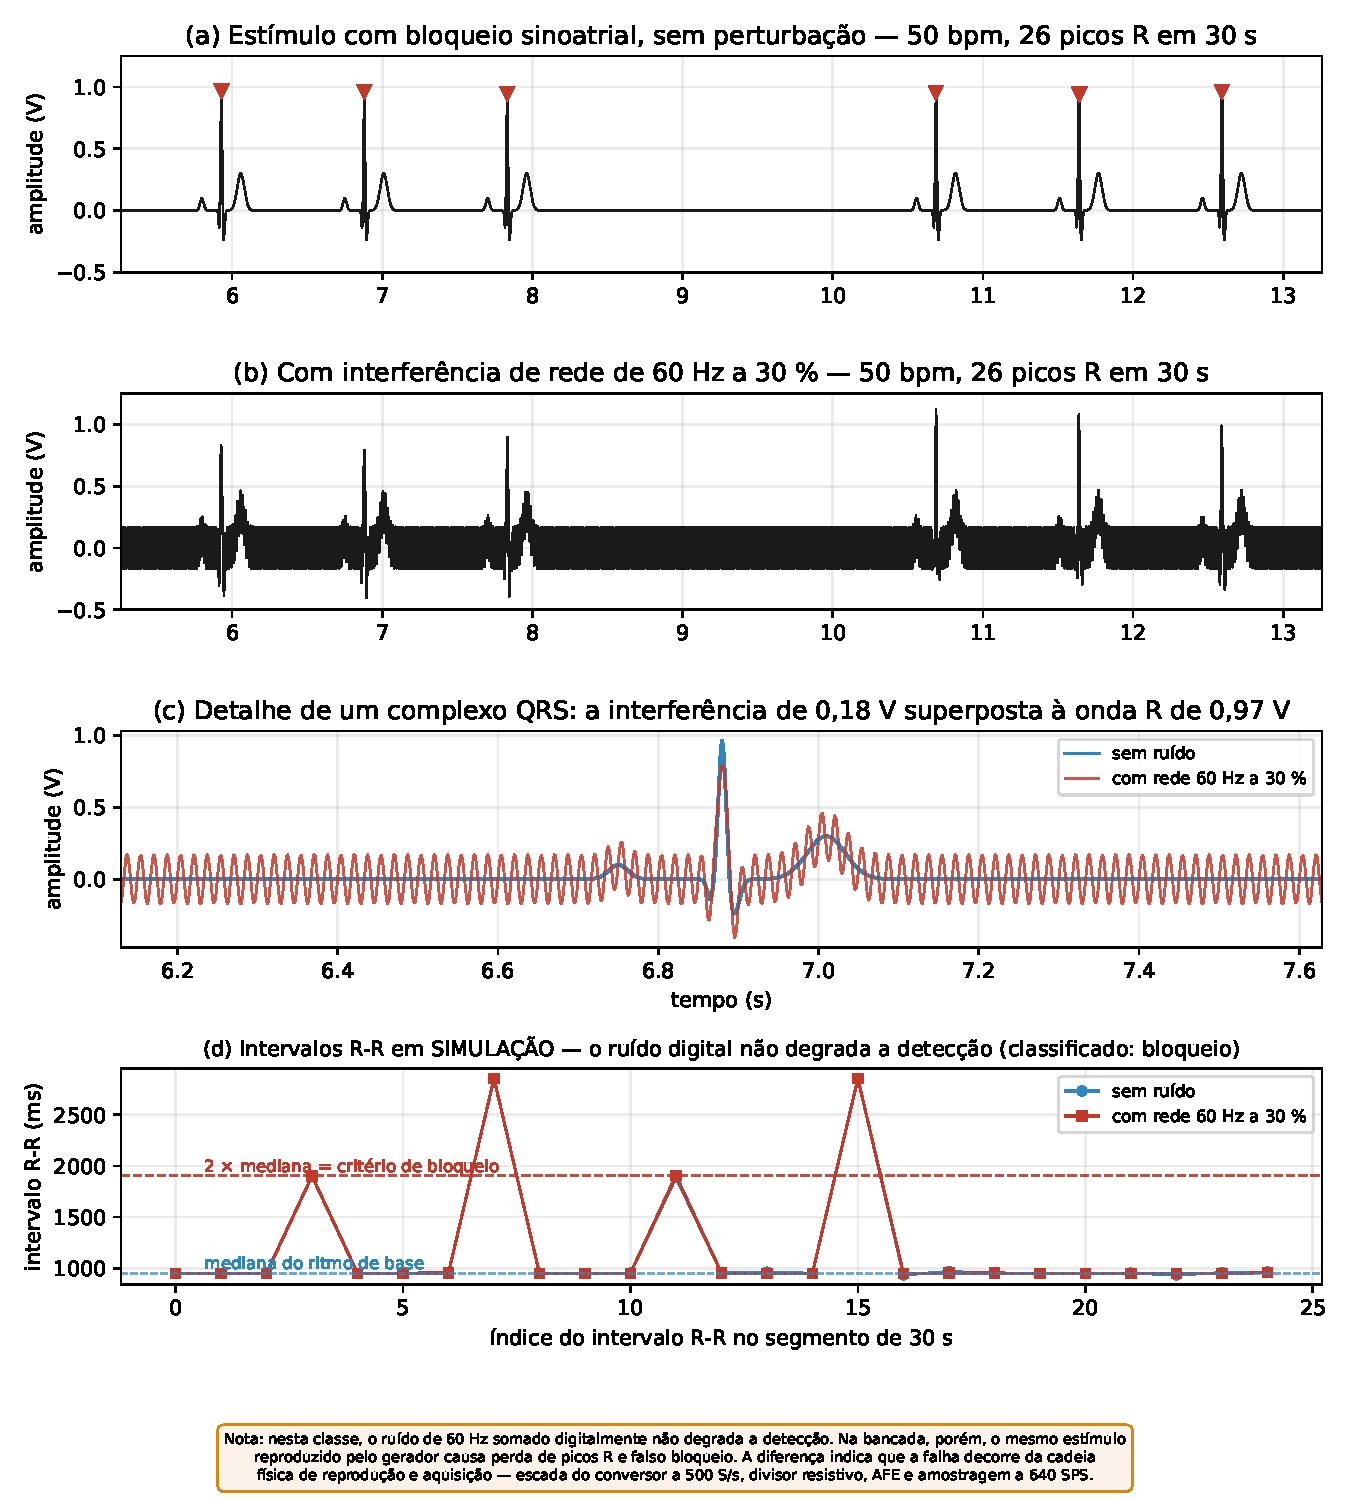
\includegraphics[width=0.92\linewidth]{assets/figura_rede30_bloqueio.pdf}
\caption{Estímulo com bloqueio sinoatrial sob interferência de rede a 30\,\%: traçados, detalhe do complexo QRS e intervalos R-R.}
\label{fig:ruidoCompletoBloqueio}
\end{figure}

\begin{figure}[htbp]
\centering
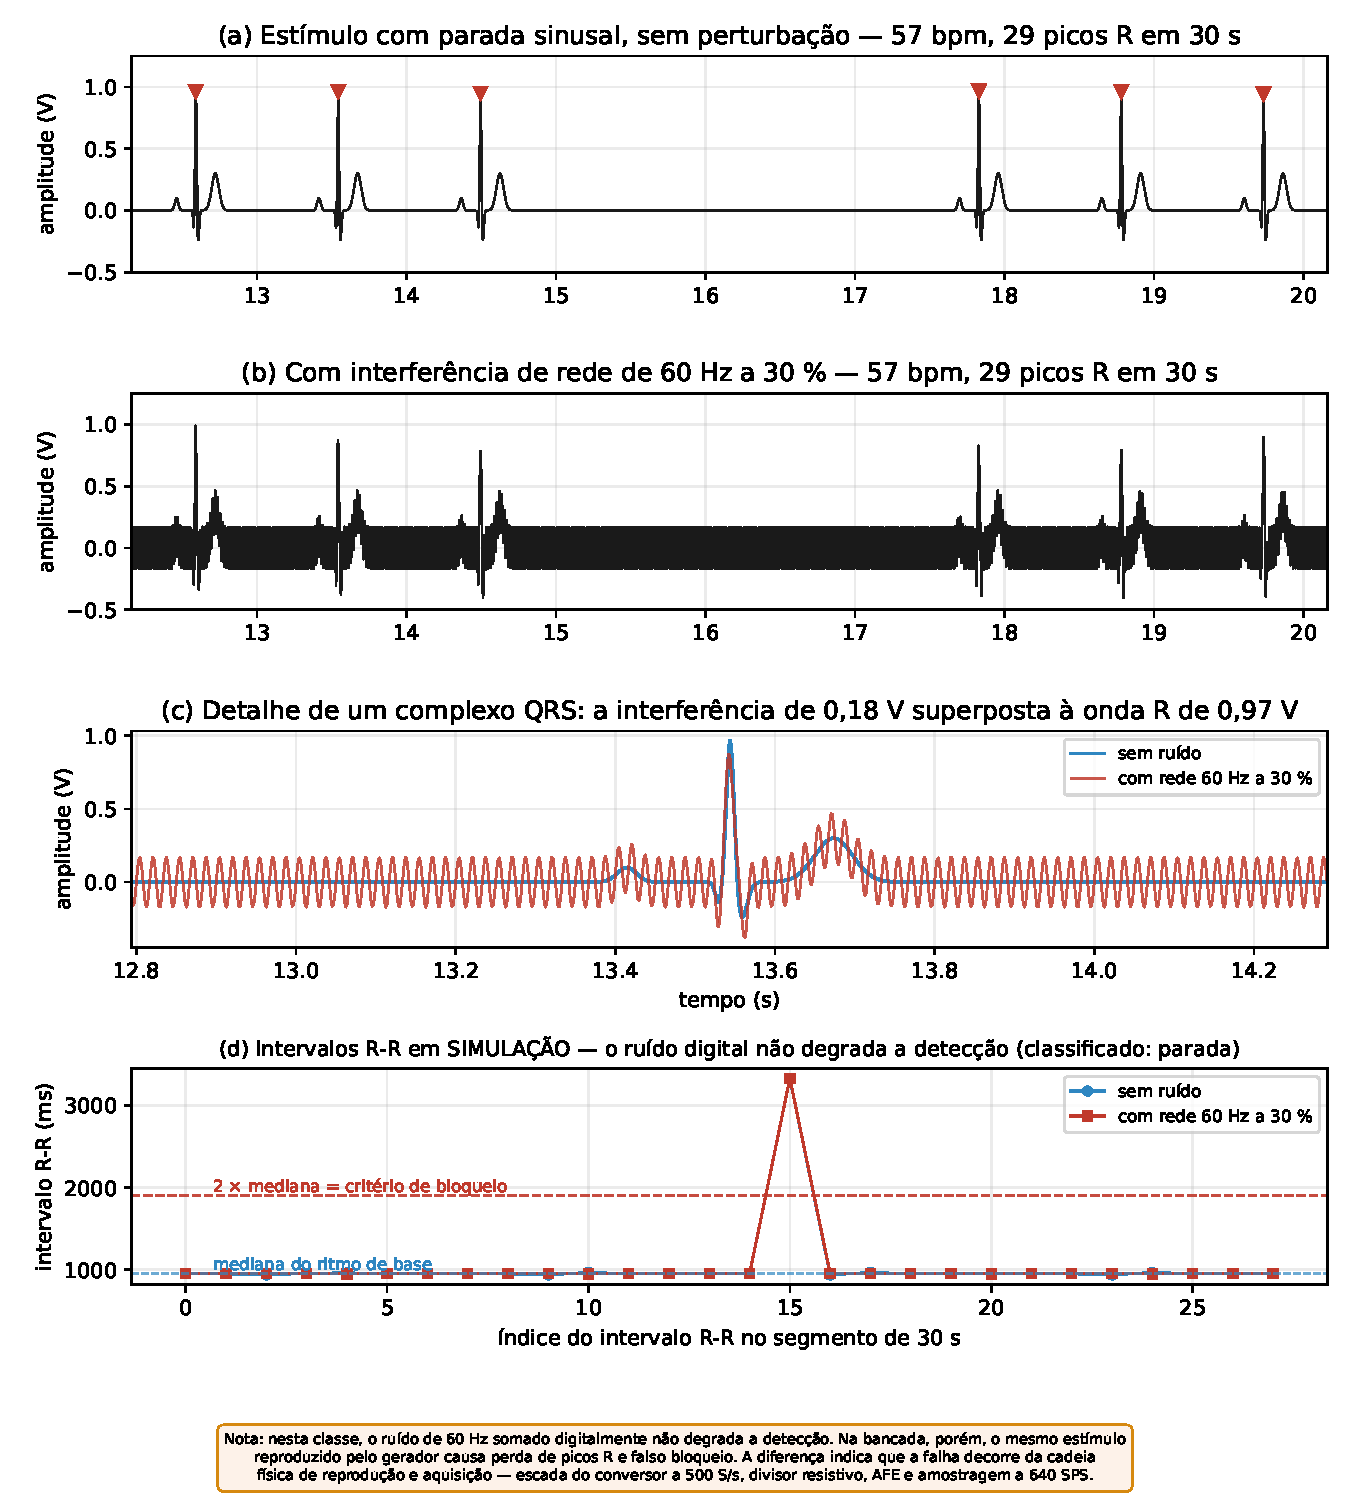
\includegraphics[width=0.92\linewidth]{assets/figura_rede30_parada.pdf}
\caption{Estímulo com parada sinusal sob interferência de rede a 30\,\%: traçados, detalhe do complexo QRS e intervalos R-R.}
\label{fig:ruidoCompletoParada}
\end{figure}

\clearpage
\section{Sinal efetivamente adquirido pelo dispositivo}
\label{ap:rawAdquirido}

A discrepância registrada na introdução deste apêndice --- a simulação não reproduz, para cinco das seis classes, a falha medida na bancada --- deixa em aberto a questão de \emph{onde}, ao longo da cadeia, a degradação se origina. A acurácia de classificação não a responde: um segmento classificado como bloqueio pode tê-lo sido porque a aquisição perdeu batimentos, porque o algoritmo não os localizou, ou por ambos.

Para dirimi-la, habilitou-se no \textit{firmware} a gravação do conteúdo do \textit{buffer} de detecção --- a sequência de amostras que o algoritmo efetivamente recebe, depois do divisor resistivo, do \acs{AFE} e da cascata de filtros digitais --- e transferiu-se esse conteúdo pela interface serial. Adquiriram-se três segmentos de 30~s do mesmo estímulo normal: sem perturbação, sob interferência de rede de 60~Hz a 30\,\% e sob ruído aleatório de idêntica amplitude. A Figura~\ref{fig:rawAdquirido} apresenta um recorte de 10~s dos três.

\begin{figure}[htbp]
\centering
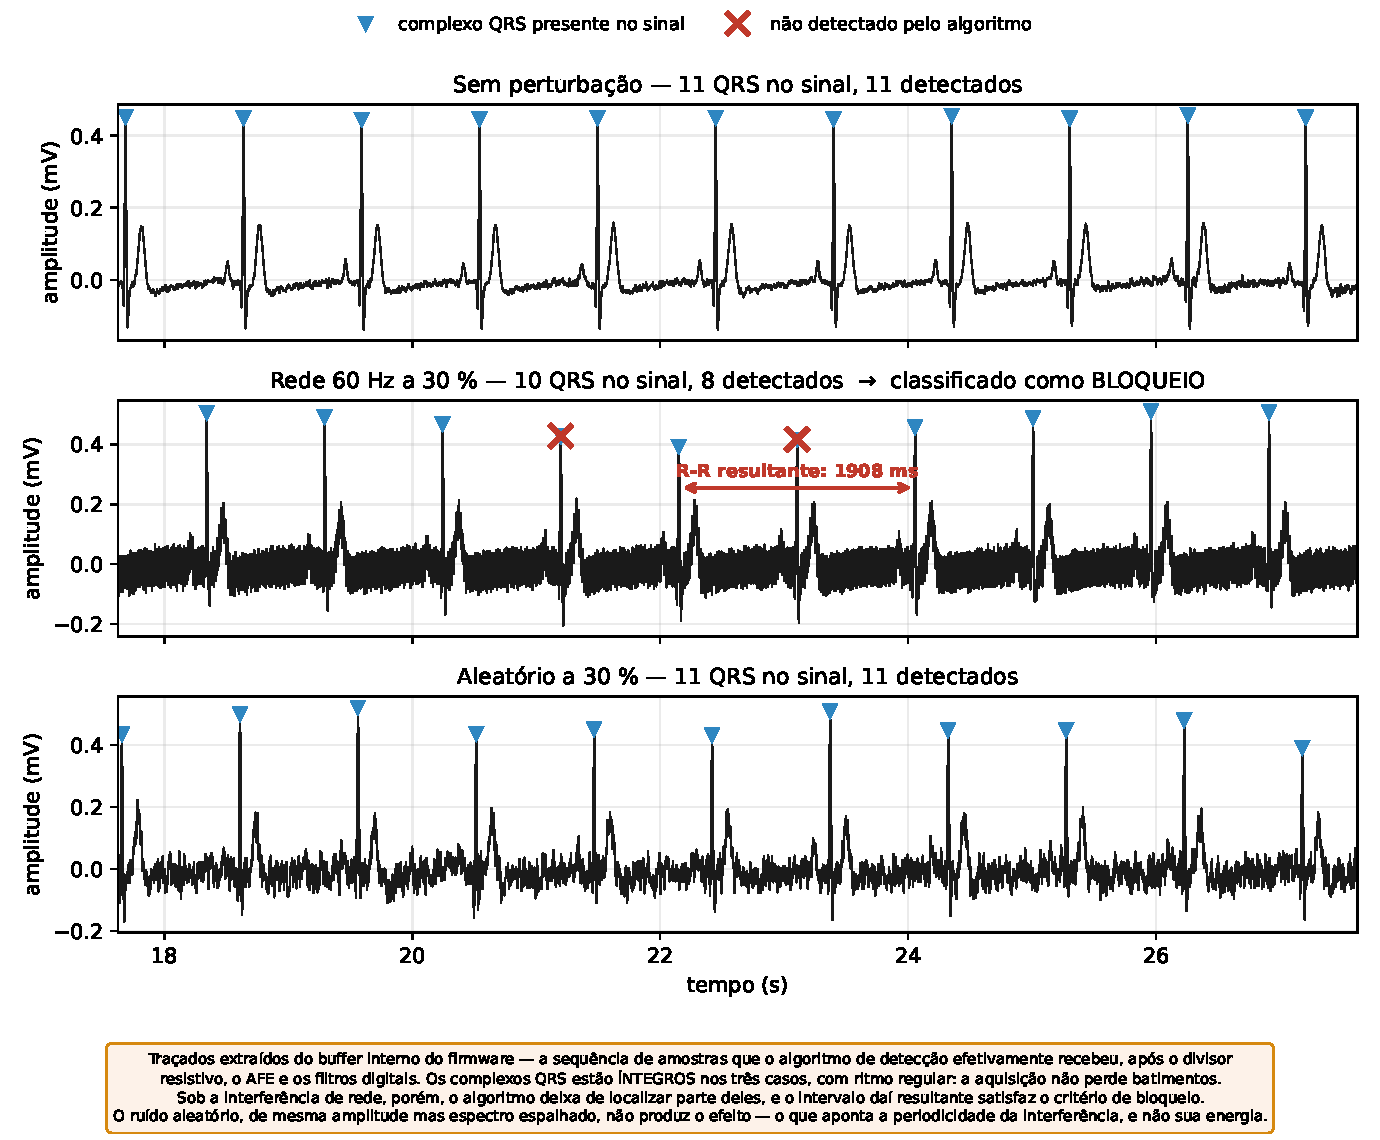
\includegraphics[width=\linewidth]{assets/figura_raw_adquirido.pdf}
\caption{Sinal de \acs{ECG} tal como recebido pelo algoritmo de detecção, sob três condições de estímulo. Os triângulos assinalam os complexos QRS presentes no sinal; as cruzes, aqueles que o algoritmo não localizou. Sob a interferência de rede, os complexos permanecem íntegros, mas dois deles deixam de ser detectados no recorte exibido, e o intervalo R-R daí resultante --- 1.908~ms, o dobro da mediana de 952~ms --- satisfaz o critério de bloqueio sinoatrial.}
\label{fig:rawAdquirido}
\end{figure}

O resultado é inequívoco. Nas três condições, os complexos QRS encontram-se íntegros no sinal adquirido, e o intervalo R-R mediano permanece em 952~ms --- idêntico ao do estímulo sem perturbação. A cadeia de aquisição, portanto, \textbf{não perde batimentos} sob nenhuma das perturbações ensaiadas, inclusive na amplitude máxima. O que difere entre os três casos é a capacidade do algoritmo de \emph{localizar} os complexos: sob a interferência de rede, foram reconhecidos 27 dos 32 presentes no segmento; sob ruído aleatório de mesma amplitude, todos os 31.

A explicação está no método de detecção. O algoritmo reaproveitado localiza os complexos pela operação de diferenças (Seção~\ref{sec:deteccaoBorda}), que opera sobre a derivada do sinal e pareia máximos com mínimos locais. Uma senoide de 60~Hz possui derivada da mesma ordem de grandeza que a do complexo QRS, de modo que o pareamento de extremos se desorganiza e o limiar adaptativo se desloca; o ruído aleatório, de espectro espalhado, não concentra energia em nenhuma frequência específica e não produz o mesmo efeito. Não é, pois, a amplitude da perturbação que compromete a detecção, mas sua periodicidade.

Duas consequências decorrem dessa constatação. A primeira é de atribuição: a limitação sob interferência de rede pertence ao algoritmo de detecção de picos, reaproveitado de \citet{moraesFirmwareECG}, e não à cadeia de aquisição desenvolvida nesta dissertação, cujo desempenho se mostrou íntegro na condição mais severa ensaiada. A segunda é de encaminhamento: o aprimoramento pertinente não está no estágio de filtragem --- cuja tentativa, o filtro rejeita-faixa avaliado na Seção~\ref{sec:resNotch}, não trouxe ganho líquido ---, mas na substituição do método de localização dos complexos por outro menos sensível à interferência periódica, alternativa já registrada entre os trabalhos futuros no Capítulo~\ref{chap:conclusoes}.
